\chapter{Results} \label{ch:conclusions}

In order to gauge the practical benefit of the GPU-based FDTD implementation, we compare execution time  of GPU and CPU implementations. We measure performance as a function of total execution time for a given domain size and number of time steps or frames, as well as number of cell operations completed per second. 

\begin{figure}[H]
	\centering
	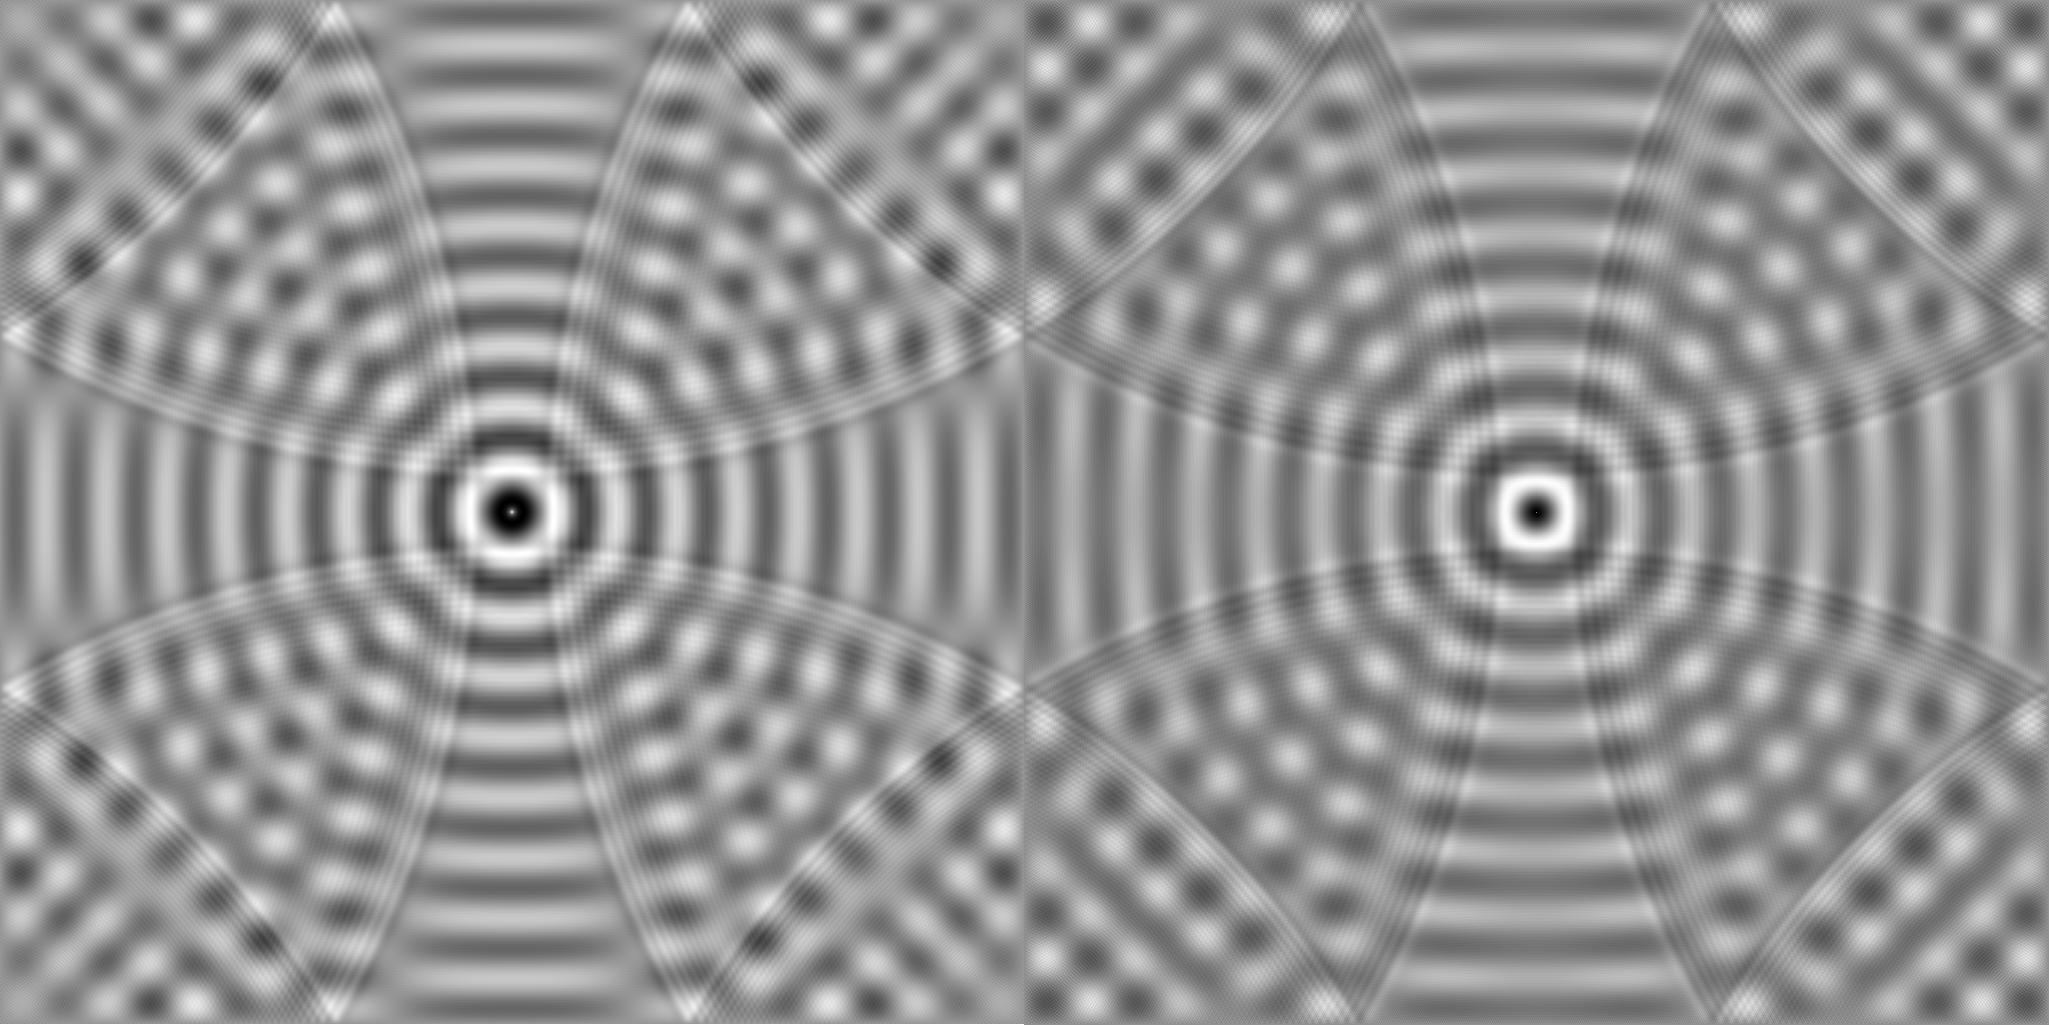
\includegraphics[width=\textwidth,keepaspectratio]{point-source-comparison.jpg}
	\caption{GoLightly (left) vs Meep (right) output for a ${TM}_Z$ simulation with a single point source and Dirichlet boundary.}
	\label{fig:pointSourceComparison}
\end{figure}

\section{Test Environment}

Tests were performed on a 2015 Dell XPS 9550 with 32GB of RAM, Intel i7 2600 CPU and NVIDIA 960M GPU with 640 cores and 1GB of VRAM. GoLightly GPU tests were executed under Microsoft Windows 10, while Meep CPU tests were run under Ubuntu Desktop version 16.04.
 

\section{Performance Metrics}

Metrics were calculated using domain sizes ranging from 128x64 to 8192x4096 over 5000 frames. (In this case, a frame represents a complete time step wherein all $E$ and $H$ fields are updated.) For benchmarking purposes, the visualizer was disabled.


\begin{figure}[H]
	\centering
	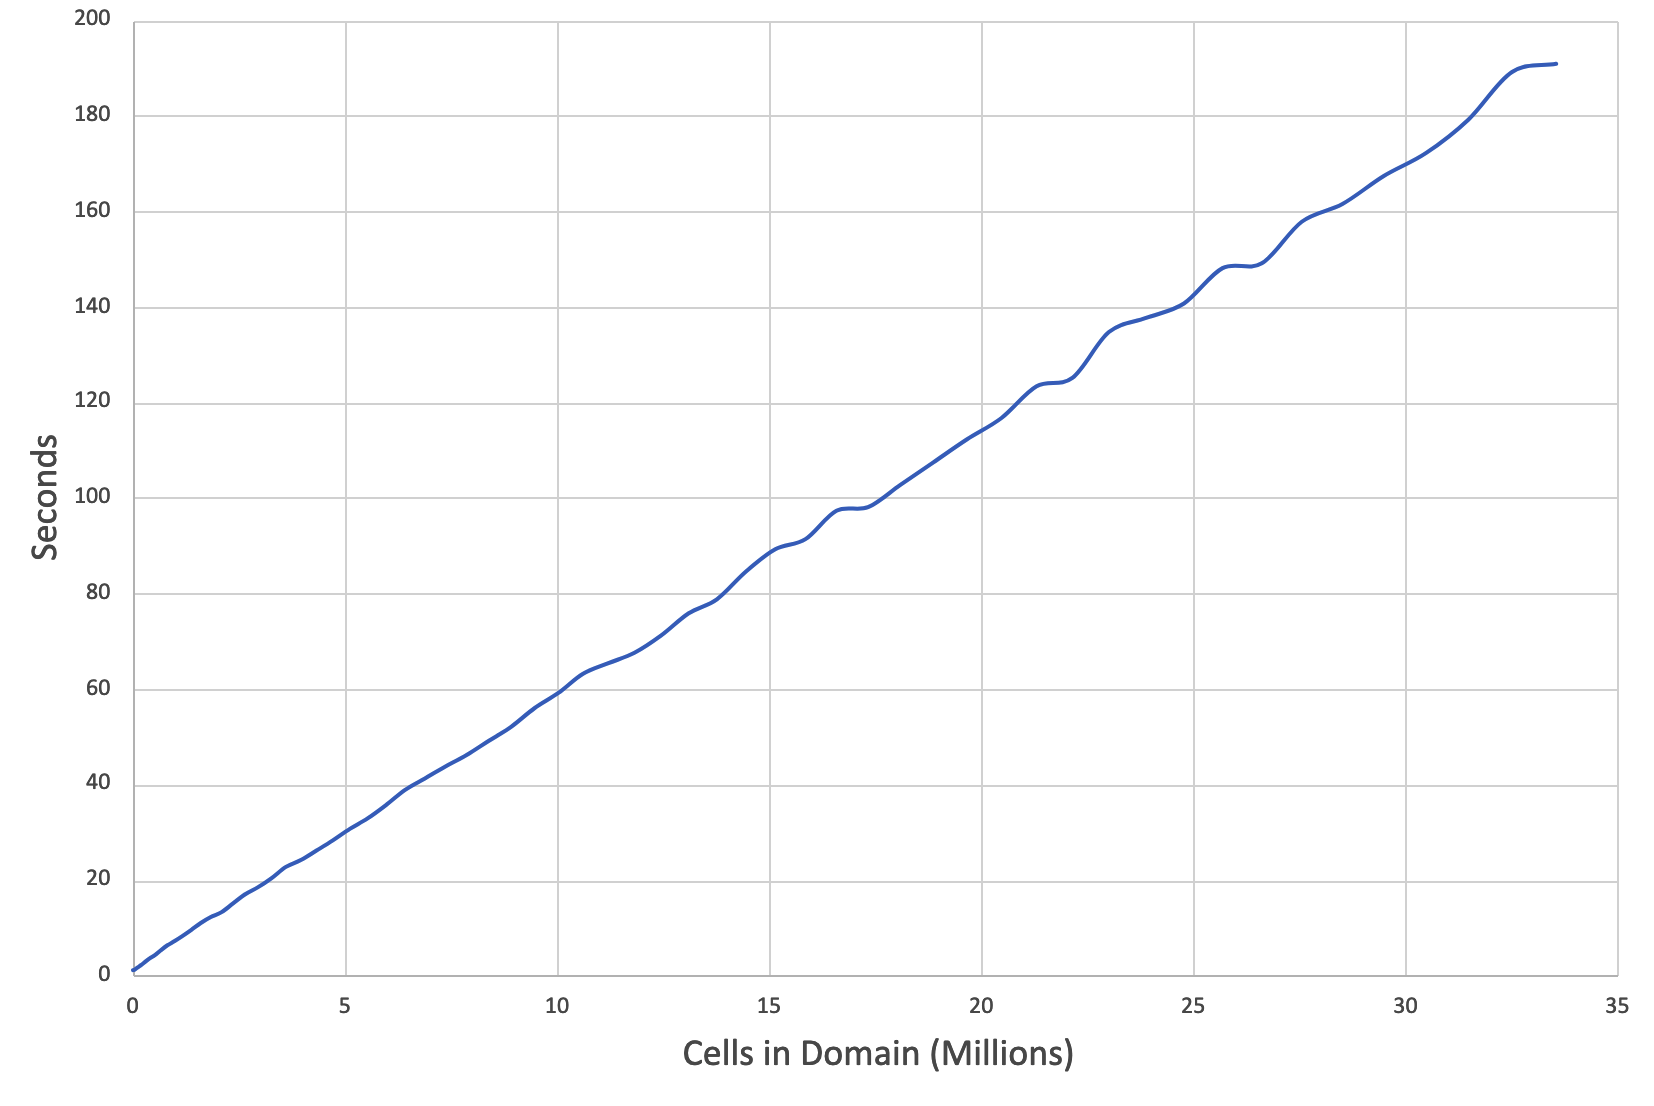
\includegraphics[width=\textwidth,
	keepaspectratio]{gpu_seconds_vs_domain_size.png}
	\caption{GoLightly: seconds for 5000 frames with the given domain size}
	\label{fig:gpuTimeVsDomainSize}
\end{figure}

\autoref{fig:gpuTimeVsDomainSize} shows that computation time increases linearly as a function of simulation domain size.


\begin{figure}[H]
	\centering
	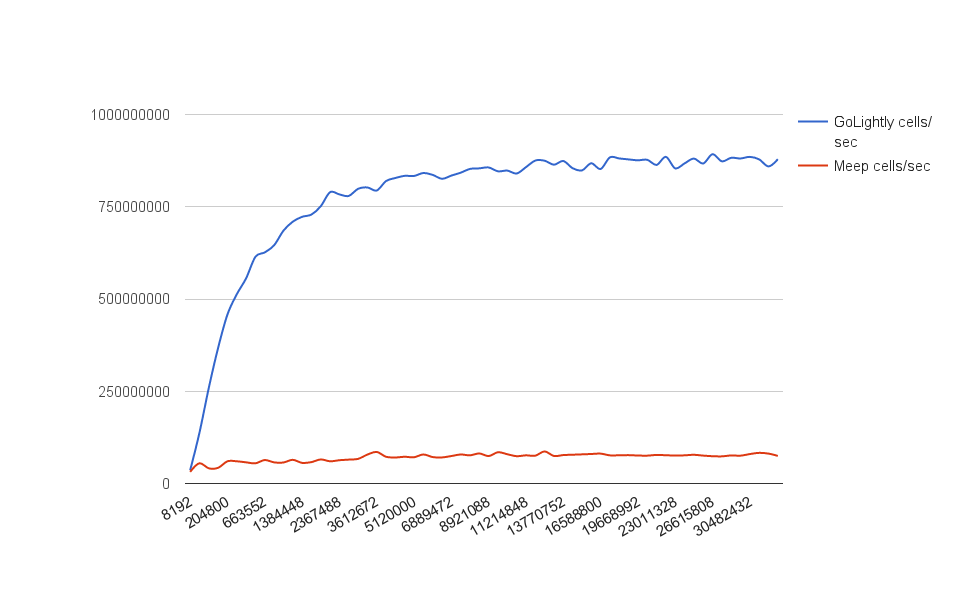
\includegraphics[width=\textwidth,
	keepaspectratio]{cells-per-second.png}
	\caption{GoLightly: Completed E and H updates per second}
	\label{fig:gridSizeVsComputeTime}
\end{figure}

Note that GPU throughput (represented in \autoref{fig:gridSizeVsComputeTime} as “cell” operations per second) increases dramatically as the domain size increases, until GPU initialization overhead is overcome by computation time.

\begin{figure}[H]
	\centering
	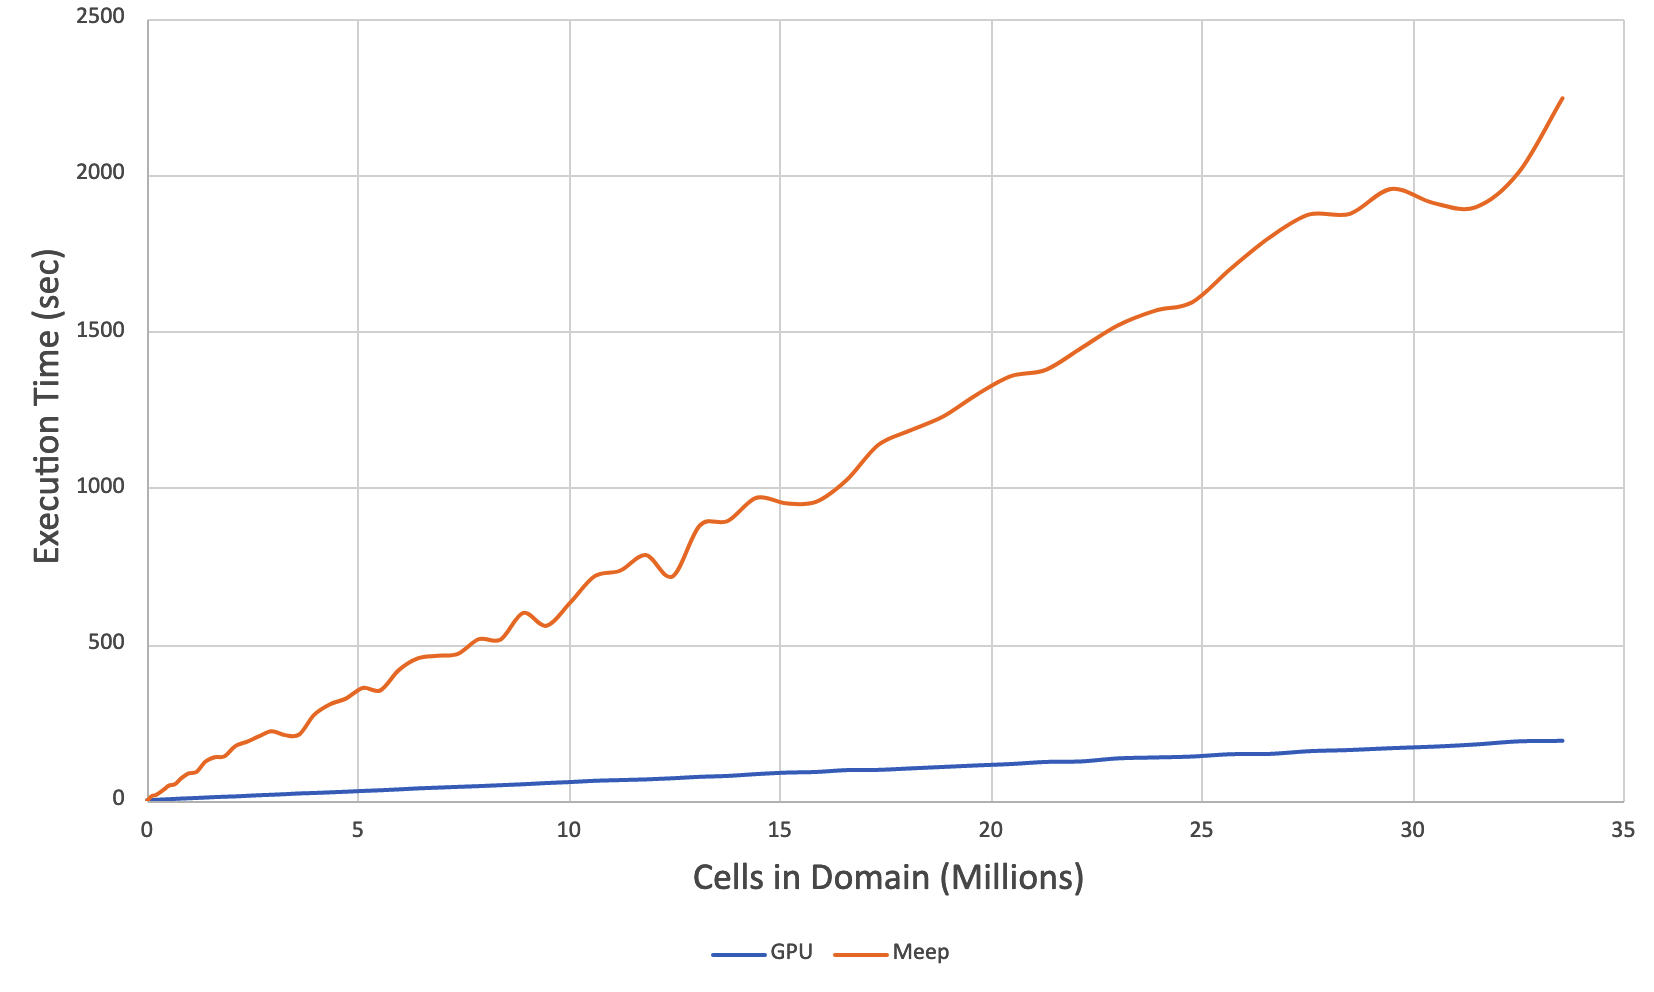
\includegraphics[width=\textwidth,
	keepaspectratio]{gpu-vs-meep.png}
	\caption{GoLightly vs Meep: Seconds for 5000 frames with X cells and 10 PML layers}
	\label{fig:gpuVsMeep}
\end{figure}

In \autoref{fig:gpuVsMeep}, note some CPU performance variance near the middle and end of the graph. Multiple runs consistently exhibited this behavior. While the cause of these variances is not clear, it has been reproduced on different hardware and operating system versions. 
This may be caused by several factors, including:

\begin{itemize}
	\item Memory alignment. When reading or writing from memory, CPUs perform best when dealing with boundary-aligned data. The dimensions of the simulation domain affect this alignment.
	\item Multi-tasking preemption. In multitasking operating systems such as Linux or Windows, background tasks may preempt foreground tasks, resulting performance degradation. 
	\item Memory latency. Relatively slow access to out-of-core memory may cause a pipeline stall.	
\end{itemize}


\begin{figure}[H]
	\centering
	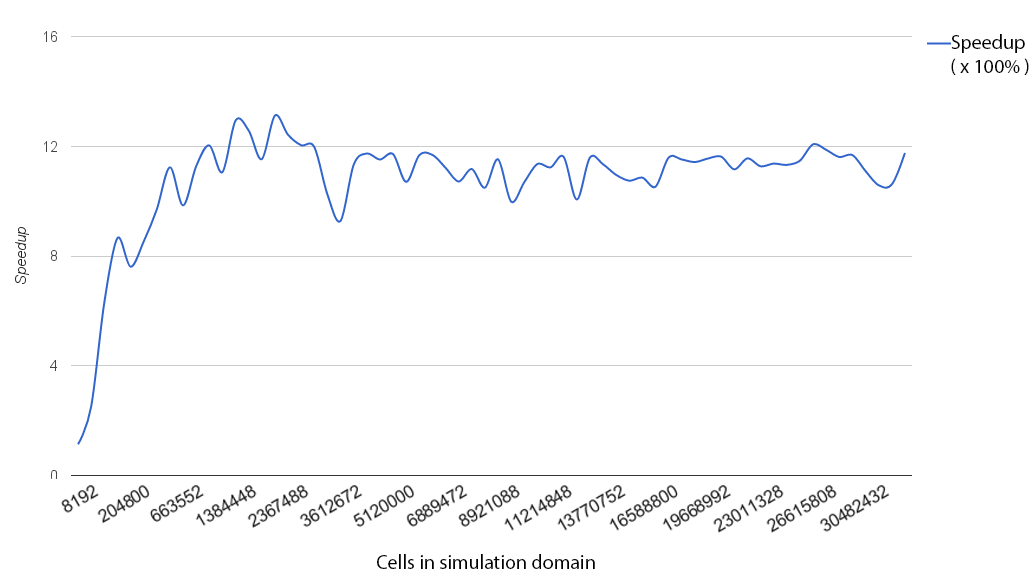
\includegraphics[width=\textwidth,
	keepaspectratio]{gpu-vs-meep-speedup.png}
	\caption{Speedup - Meep Time / GoLightly Time}
	\label{fig:gpuVsMeepSpeedup}
\end{figure}

\autoref{fig:gpuVsMeepSpeedup} shows a speedup ranging from 1.2 to 12, depending on the domain size. At lower resolutions, the overhead of initializing assets on the GPU and copying results to the CPU can take more time than the simulation. In that case, the CPU may outperform the GPU solution.

\section{Optimization and Enhancements}

Although a 1100\% speed increase is significant, there is much room for improvement. GPUs provide different memory spaces that vary in capacity and access speed. In addition to global device memory, each warp\footnote{A wave, wavefront or warp is a group of 32 (NVIDIA) or 64 (AMD) threads allocated to a common stream processor unit.} has shared memory\footnote{Shared memory is physically local to the ALU and accessible by all threads within the warp.} and local memory\footnote{Each thread has local memory which is not accessible to any other thread.}.

While global memory is the most flexible and plentiful - typically on the order of gigabytes on current generation-hardware - it is also the slowest. 

Shared memory is common to all threads in a wave. It can be used for intra-thread synchronization and resource sharing, and is significantly faster than global memory.

Finally, local memory provides thread-local storage. Local memory provides the lowest latency of all memory spaces.

In its current form, GoLightly makes little use of shared or local memory. Modifying the application to take advantage of those would likely improve performance.







